\begin{figure}[t]
\centering
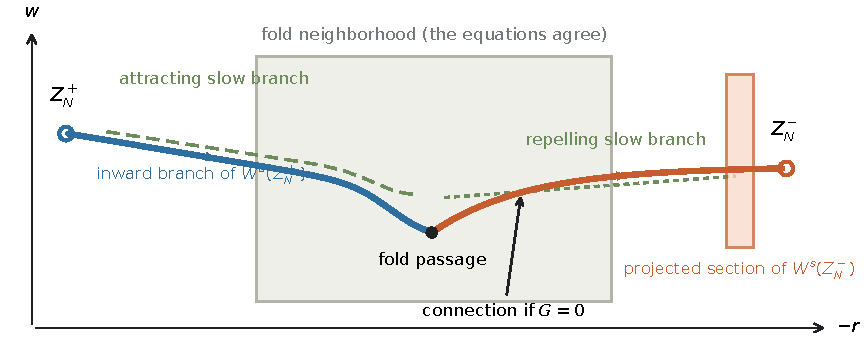
\includegraphics[width=\textwidth]{figures/connection-geometry.pdf}
\caption{Geometry of the conditional connection statement.  \textbf{(a)}
Schematic projection into the collective coordinates \((-r,w)\).  The dashed
green curve is the frozen critical curve, with its attracting branch on the
left and repelling branch on the right.  The solid blue curve represents the
specified orbit at a zero of \(G\); the black arrowheads indicate forward
time.  In these
coordinates the fold is a local maximum.  The gray strip marks
\(\abs r\leq r_{\rm loc}\), where the original and modified recovery laws
agree, and \(\Sigma_0=\{X=0\}\) is the common phase condition.  \textbf{(b)}
Schematic two-dimensional slice of the Banach-manifold chart on
\(\mathcal M_{\Sigma_0}^2\), shown at a nearby parameter with \(G\ne0\).
The incoming point \(A^0=(\psi_A,u_A)\) and the stable-manifold section
\(u=F^-(\psi)\) define \(G=u_A-F^-(\psi_A)\).  The displayed gap
illustrates this defining function; it collapses at the connection shown in
panel~\textbf{(a)}.  The figure does not prove existence or establish the
global invariant-manifold hypotheses, and positions and distances are not
quantitative.}
\label{fig:connection-geometry}
\end{figure}
